\section{Introducción al Sistema de Manejo de Eventos de \nombreFramework}
Uno de los principales objetivos de este proyecto es que una red de Petri
se encargue del manejo completo de la concurrencia y el asincronismo de un
sistema informático. Para logralo, se implementó el monitor de petri por software descripto en la
sección \emph{\color{red} CITA REQUERIDA seccion monitor}.
El mismo está basado en la implementación previa realizada en \cite{codegen}.
Este monitor permite delegar la concurrencia y asincronismo del
sistema a una red de Petri. Un ejemplo de uso exitoso se describe en
\cite{Bentivegna-Ludemann}.

Sin embargo, la utilización directa del monitor es engorrosa y genera un
alto grado de acoplamiento entre el software de usuario y la red de Petri. La
red queda asociada directamente a los eventos del mundo real. La principal
desventaja de tener un sistema acoplado a la red de Petri está dada por la
reducción de la escalabilidad del sistema. Esto se debe a que la sustitución de la red (o
su modificación) implica también un cambio en el código del software,
dificultando un proceso de desarrollo iterativo o por etapas. Otra gran
desventaja es que impide la realización de redes de Petri genéricas, más
versátiles, útiles para resolver diferentes problemas de
características similares.

Otro objetivo del proyecto consiste en la facilidad de uso. Como se explicó
anteriormente, la utilización directa del monitor es complicada y puede
favorecer a la generación de errores, ya que deben crearse todos los hilos de
ejecución y deben programarse los disparos de transición de forma manual en el
código. Ante un cambio en la red de petri deben modificarse algunos o todos los
disparos de transición distribuidos a lo largo del código, pudiendo llevar a
una incorrecta sincronización de los hilos si no se realiza con especial precaución.

Finalmente, otro objetivo importante es el de crear una herramienta que permita
al usuario estructurar el proyecto utilizando patrones de diseño de forma
simple. En el caso de utilizar el monitor de forma directa, el diseño del
software queda en manos del usuario desarrollador. Esto significa que la
decisión de utilizar o no patrones de diseño es tomada por el usuario. De
esta manera se desaprovecha la oportunidad de reutilizar ciertos aspectos de
diseño que se consideran pertinentes. Por ejemplo el patrón command descripto en
\cite{chimp}, o algunas caracteristicas similares a un diseño MVC que se pueden
observar en los sistemas sincronizados por Petri. Este último ejemplo se explica
con mayor detalle en la sección \emph{\color{red} CITA REQUERIDA Patrón MVC
en el framework?}.

Como resultado de este análisis, se llegó a la conclusión de que se puede
aprovechar mejor el potencial del monitor si se encuentra embebido en un
framework que se encargue de desacoplar el código de usuario de la lógica de
disparos y de sincronización de hilos. 
Una conclusión de similares características se desprende de
\cite{Bentivegna-Ludemann}, donde los autores expresan: ``La debilidad encontrada en el proceso de elaboración del
software, es que resultó problemático vincular los hilos con las transiciones de
la RdP. Esto se debe a que, en el código de las acciones, quedó embebida la
relación de éstas con las transiciones. Por lo cual, queda en evidencia que es
necesaria la existencia de un framework para automatizar y facilitar la
vinculación entre eventos, acciones y transiciones.''


\section{Sincronización por Red de Petri a través de Eventos}
Se puede definir a un sistema desarrollado utilizando el monitor como un
programa de software que intercambia eventos con la red de Petri y con su
entorno físico.

\begin{figure}[h]
	\centering
	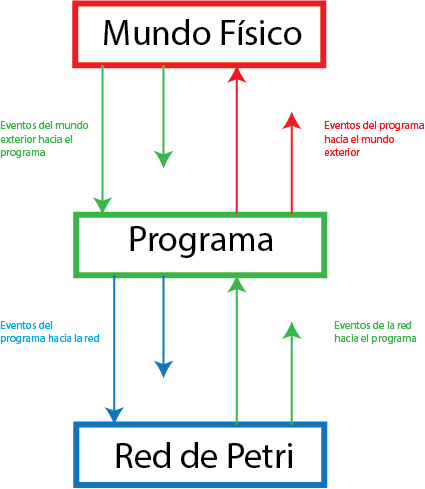
\includegraphics[width=75mm]{eventos_petri-programa-mundo}
	\caption{Intercambio de eventos en un programa sincronizado por Red de Petri}
	\label{fig:eventos_petri-programa-mundo}
\end{figure}

El programa puede acceder a hardware del mundo físico, ya sea para realizar una
acción (por ejemplo utilizando actuadores) o  para obtener eventos del mundo
exterior y comunicarselos a la red de Petri (utilizando sensores, por ejemplo).

La red toma los eventos del mundo exterior y los combina con condiciones del
problema y de sincronización para emitir eventos de salida hacia el programa. La
red es básicamente un procesador de eventos.\cite{chimp}

Este concepto se amplía en la sección Eventos Físicos y Eventos
Lógicos de \cite{chimp}. En esta sección se distingue la existencia de los dos
tipos de eventos mencionados, y se los define como:
  \begin{itemize}
    \item Eventos Lógicos: eventos que son comprensibles por el monitor de
    redes de Petri, y están inherentemente asociados a transiciones de la red
    misma y sus colas.
    \item Eventos Físicos: suceden en el mundo físico y representan sucesos del
    dominio del problema
  \end{itemize}

Tras la incorporación del concepto de eventos lógicos y físicos, los autores
proponen en \cite{chimp} un diagrama de arquitectura de alto nivel como el de
la Figura~\ref{fig:eventos_fisicos-logicos}.

\begin{figure}[h]
	\centering
	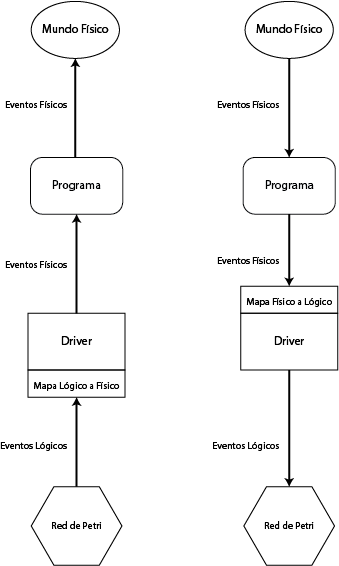
\includegraphics[width=75mm]{eventos_fisicos-logicos}
	\caption{Arquitectura con Eventos Físicos y Lógicos}
	\label{fig:eventos_fisicos-logicos}
\end{figure}

Luego de estudiar los ejemplos desarrollados utilizando Chimp Java Driver por
sus creadores en \cite{chimp}, se logró determinar que la clasificación de los
eventos en dos tipos no es suficiente para explicar la comunicación en un
sistema de estas características. Esto se debe a que los eventos físicos
representados previamente en Figura~\ref{fig:eventos_fisicos-logicos} abarcan dos
tipos de eventos. Uno de ellos está efectivamente relacionado con el hardware o
software externos al sistema (mundo físico). El otro tipo de eventos está
relacionado con el manejo de las acciones que van a realizar dichos elementos
del mundo exterior, el cual se realiza a través del software del sistema.

A partir de lo expuesto en el párrafo previo, se propone una nueva clasificación
de eventos:

\begin{itemize}
    \item Eventos Lógicos: eventos que son comprensibles por el monitor de
    redes de Petri, y están inherentemente asociados a transiciones de la red
    misma y sus colas. Este tipo de eventos se comunica utilizando las
    interfaces proporcionadas por el monitor de redes de Petri.
    \item Eventos de Acción \emph{\color{red} VER NOMBRE}: Evento intermedio
    entre los eventos físicos y lógicos. Este tipo de evento debe ser
    comprendido por un módulo del framework encargado de manejarlos. Sirven para
    desencadenar acciones de software, que en última instancia se comunican con
    el mundo exterior a través de los eventos físicos y con la red de petri a
    través de los eventos lógicos. Son una traducción intermedia entre los
    eventos físicos y lógicos, necesaria para desacoplar la red de Petri del
    mundo Físico y permitir la inversión de control descripta en la sección de
    frameworks \emph{\color{red} CITA REQUERIDA: seccion frameworks}.
    \item Eventos Físicos: suceden en el mundo físico y representan sucesos del
    dominio del problema. Este tipo de eventos se comunican a través de las
    interfaces que ofrezca el elemento del mundo exterior y el lenguaje Java.
    Por ejemplo pueden comunicarse a través de Event Listeners, mecanismos
    de IPC, Sockets, Serial, Bluetooth, etc.
\end{itemize}

Teniendo en cuenta esta nueva clasificación de los eventos presentes en el
sistema, se propone una nueva arquitectura de alto nivel
(Figura~\ref{fig:arquitectura_petri-manejador-acciones-mundo}). El framework a
realizar en este trabajo tiene requerimientos de inversión de control. De esta forma, el nuevo diagrama incorpora estos requerimientos en su diseño, además de
la nueva clasificación eventos.\emph{\color{red} Ver: seccion frameworks, inversión de control}

\begin{figure}[h]
	\centering
	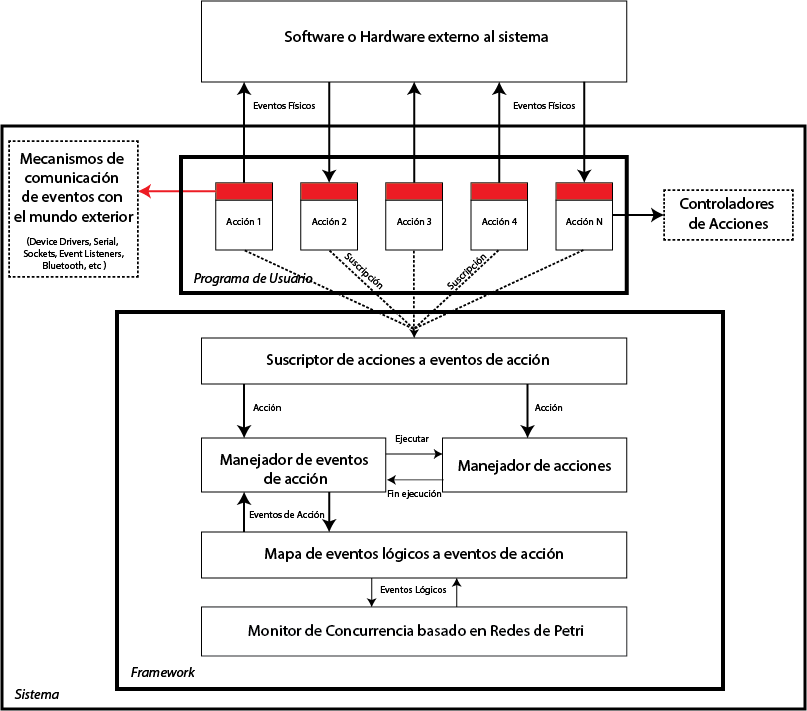
\includegraphics[width=120mm]{arquitectura_petri-manejador-acciones-mundo}
	\caption{Diagrama de Arquitectura de Alto Nivel}
	\label{fig:arquitectura_petri-manejador-acciones-mundo}
\end{figure}

\subsection{Componentes de un sistema desarrollado con \nombreFramework}
Como puede apreciarse en la
Figura~\ref{fig:arquitectura_petri-manejador-acciones-mundo}, un sistema
desarrollado con \nombreFramework puede dividirse en tres partes a nivel de arquitectura.
\begin{itemize}
\item Existe un monitor de redes de Petri, encargado de analizar el
cumplimiento de las condiciones para la ejecución de ciertas partes de código
(acciones). 
\item La segunda parte esta compuesta por un subsistema manejador de eventos de
acción y un subsistema manejador de ejecución de acciones. Estos subsistemas
estan conectados con el monitor de redes de Petri y utilizan un mapa para 
intercambiar eventos entre sí. De esta forma se permite la separación de los
eventos lógicos y eventos de acción del sistema.\\
A su vez, presenta un suscriptor de acciones, que ofrece al usuario las
interfaces necesarias para asociar una acción a un evento de acción.\\
Toda esta etapa actúa como intermediaria entre el
código del usuario y el monitor de redes de Petri, permitiendo desacoplar la
red de Petri del código de usuario.
\item Por último, el programa de usuario contiene todas las acciones
concretas a realizar, con sus correspondientes suscripciones a eventos
programáticos. Dichas acciones pueden comunicarse con el mundo exterior de
cualquier forma deseada por el usuario desarrollador. Por esta razón, el manejo
de los eventos físicos es responsabilidad del usuario.
\end{itemize}


\subsection{Condiciones de Ejecución en un Programa de Software}
Un sistema de software puede ser visto como una secuencia de acciones que son
ejecutadas ante el cumplimiento de determinadas condiciones. Desde el punto de
vista del programa que analiza dichas condiciones, se pueden clasificar
en síncronas y asíncronas.
  \begin{itemize}
	\item Síncronas: Por ejemplo, condiciones booleanas derivadas del estado del
		sistema que realizan cambios en el flujo de instrucciones del mismo (saltos
		condicionales).
	\item Asíncronas: Por ejemplo, eventos provenientes del mundo exterior o
		señales/mensajes entre hilos/procesos.
  \end{itemize}
El objetivo de este trabajo es utilizar redes de Petri para controlar la
ejecución de todas aquellas acciones que respondan a estos tipos de condiciones.
De esta forma, será el monitor de redes de Petri quien analice las condiciones y
explicite el estado del sistema. De esta manera, queda bajo consideración de la red:
\begin{itemize}
  \item Disparo de eventos provenientes de sistemas externos, que pueden llegar
  en cualquier instante de tiempo y sin un orden preestablecido. Los estados
  locales de la red se mantienen en causalidad de las acciones ejecutadas con
  anterioridad. El monitor es el encargado de mantener el estado lógico del
  sistema.
  
  \item Condiciones de sincronización para el ordenamiento de la ejecución de
  acciones en el tiempo. 
  
  \item Condiciones impuestas por el dominio del problema. El monitor es el
  encargado de impedir la ejecución de una acción hasta que la misma pueda ser
  realizada sin riesgos de sufrir problemas de concurrencia.
\end{itemize}

Por su lado, el sistema de ejecución de acciones se encarga de ejecutar dichas acciones cuando
el monitor de red de Petri lo dispone. El sistema de manejo de eventos de acción
es el encargado de mantener la comunicación entre el monitor y el sistema de
ejecución de acciones. El monitor es el encargado de avisar cuando una acción
debe comenzar y, por otro lado, cuando una acción concluye se le da aviso al
monitor.

Finalmente La definición y el desarrollo de dichas acciones, y su
asociación a los eventos de acción correspondientes quedan a cargo del usuario
desarrollador. Se resalta el hecho de que el usuario no decide en qué momento se
ejecuta la acción, ya que con el fin de lograr la inversión de control,
dicha responsabilidad es otorgada al monitor de redes de Petri.

